\documentclass{LIKE}

\definecolor{MainGreen}{RGB}{22, 160, 133}
\definecolor{MainPurple}{RGB}{142, 68, 173}
\definecolor{MainYellow}{RGB}{211, 84, 0}
\definecolor{MainBlue}{RGB}{41, 128, 185}
\definecolor{MainRed}{RGB}{192, 57, 43}
\definecolor{MainBlack}{RGB}{44, 62, 80}

\begin{document}

\vfill
\begin{tikzpicture}[remember picture, overlay]
    \node[anchor=north west, inner sep=0] at (current page.north west) {%
        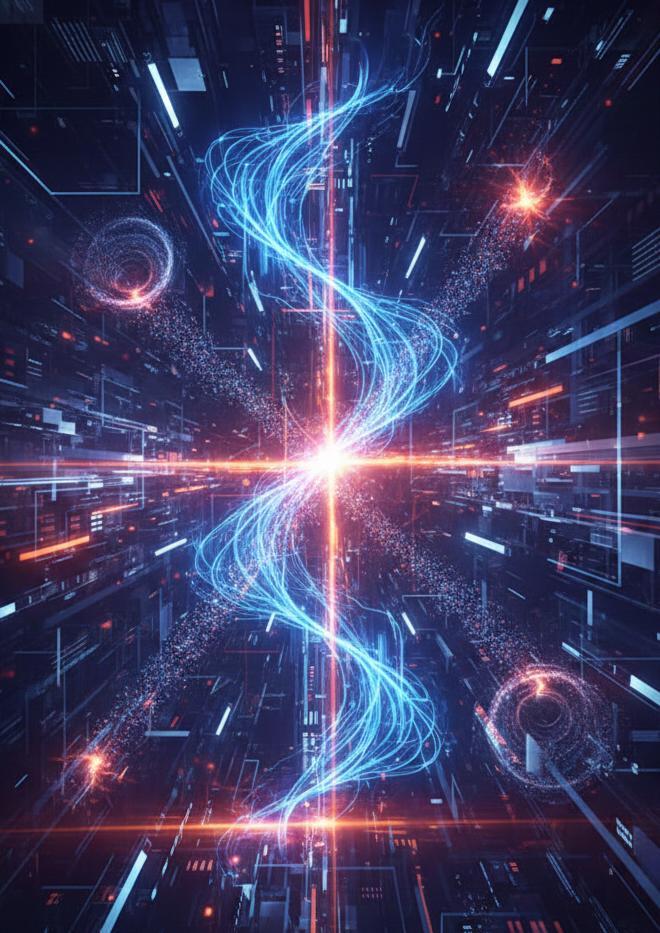
\includegraphics[width=\paperwidth, height=\paperheight]{asset/cover2.png} 
    };

    \fill[JungleGreen] 
        (current page.north east) rectangle ++(-8.0cm, -12.0cm);
    
    %\coordinate (topright) at ([xshift=-2cm, yshift=-5cm]current page.north east);
    \fill[white] 
        ([xshift=-2cm, yshift=-5cm]current page.north east) rectangle ++(-6.0cm, -7.0cm); 

    % “大学物理”大字
    \node[font=\fontsize{64}{64}\selectfont\bfseries, anchor=center] 
        at ([xshift=-5cm, yshift=-6.8cm]current page.north east) {大学};
    \node[font=\fontsize{64}{64}\selectfont\bfseries, anchor=center] 
        at ([xshift=-5cm, yshift=-9.3cm]current page.north east) {物理};

    \fill[brown!90!black] 
        ([xshift=-2cm, yshift=-12cm]current page.north east) rectangle ++(-6.0cm, -2.5cm);
        
    \node[font=\fontsize{18}{22}\selectfont\sffamily\bfseries, Gray, anchor=center] 
        at ([xshift=-5cm, yshift=-11.2cm]current page.north east) {必修~2};
    \node[font=\fontsize{24}{24}\selectfont\bfseries, black, anchor=center] 
        at ([xshift=-5cm, yshift=-13.25cm]current page.north east) {电磁学};

    \node[font=\fontsize{12}{14}\selectfont, text=black, anchor=center] 
        at ([xshift=-5cm, yshift=-2.8cm]current page.north east) {大~学~课~程~自~编~讲~义};
        
    \node[font=\fontsize{14}{14}\selectfont\sffamily\bfseries, text=white, anchor=center] 
        at ([xshift=3cm, yshift=2cm]current page.south west) {张云翼~~编};
\end{tikzpicture}

\newpage

\colorlet{maincolor}{MainBlue}
\colorlet{sidecolor}{MainBlue!50}

\setcounter{part}{2}

\setcounter{chapter}{6}

\part{电磁学}

\chapter{静电场}
\setcounter{example_counter}{1}

\section{电场强度}

\subsection{电荷的基本知识}

\subsubsection{电荷的性质}

\begin{itemize}
    \item 种类：电荷分为正、负两种，同性相斥、异性相吸
    \item 量子性：所有电荷都是元电荷$e=\SI{1.6e-19}{C}$的整数倍
    \item 电荷守恒：封闭系统的正负电荷的电量代数和保持不变
\end{itemize}

若带电体的尺度远小于研究问题，可视为\textbf{点电荷}，是一种理想模型。

\subsubsection{库仑定律}

\noindent
\begin{minipage}{0.74\linewidth}
\setlength{\parindent}{2em}
\setlength{\parskip}{0.5em}
\linespread{1.3}

真空中两个静止点电荷的作用力，与他们所带电量的乘积成正比，与距离的平方成反比，作用力的方向沿着他们的连线。

同种电荷相互吸引，异种电荷相互排斥。

\begin{formula}
    $\vec{F}=\dfrac{q_1q_2}{4\pi\varepsilon_0 r^2}\vec{e}$
\end{formula}

其中，$\varepsilon_0=\dfrac{1}{4\pi k}=\SI{8.85e-12}{C^2/(N\cdot m^2)}$称为真空介电常量。

\end{minipage}
\hfill
\begin{minipage}{0.25\textwidth}
    \vspace{-1em}
    \centering 
\includegraphics[width=\textwidth]{asset/ch7/T2.png}
\end{minipage}

\note{这与高中所学$F=k\dfrac{q_1q_2}{r^2}$的形式相同，一些教材将其形式记为$\vec{F}=\dfrac{q_1q_2}{4\pi\varepsilon_0 r^3}\vec{r}$，本质上也相同。}

\subsubsection{电力的叠加原理}

两个点电荷之间的作用力，不因第三个点电荷的存在而改变。

\subsection{电场强度}

若试探电荷$q$在电场中受力为$\vec{F}$，定义电场强度为

\begin{formula}
    $\vec{E}=\dfrac{\vec{F}}{q}$
\end{formula}

\note{电场强度是矢量，方向为正电荷受力的方向，单位为$\unit{N/C}$或$\unit{V/m}$.}

\warn{注意电场强度是电场本身的性质，与试探电荷无关。}

若已知电场强度的空间分布，则电荷$q$的受力为$\vec{F}=q\vec{E}$

\subsection{电场强度的计算}

\subsubsection{点电荷产生的电场}

\noindent
\begin{minipage}{0.75\linewidth}
\setlength{\parindent}{2em}
\setlength{\parskip}{0.5em}
\linespread{1.3}

根据电场强度的定义，点电荷产生的电场强度为

\begin{formula}
    $\vec{E}=\dfrac{q}{4\pi \varepsilon_0 r^2}\vec{e}_r=\dfrac{kq}{r^2}\vec{e}_r$
\end{formula}

\end{minipage}
\hfill
\begin{minipage}{0.23\textwidth}
    \vspace{-1em}
    \centering 
\includegraphics[width=\textwidth]{asset/ch7/T1.png}
\end{minipage}

\subsubsection{点电荷系产生的电场}

多个点电荷产生的电场，可使用\textbf{电场强度叠加原理}进行叠加计算。

电场中任一点处的总电场强度，等于各个点电荷单独存在时，在该点所产生的电场强度的矢量和。

\begin{example}{叠加法求场强}
    一根不导电的细塑料杆，$Q=\SI{3.12e-9}{C}$的正电荷均匀分布在杆上。现将塑料杆弯成近乎完整的圆，半径$R=\SI{0.5}{m}$，杆的两端有$d=\SI{2}{cm}$的缝隙，求圆心处的电场强度。
    \tcblower
    原带电体可以视为一个完整的圆和缺口处的一个点电荷的叠加。

    \vspace{-0.8em}

    \begin{center}
        
\includegraphics[width=0.4\textwidth]{asset/ch7/T3.png}
    \end{center}

    \vspace{-0.8em}
    
    而完整的圆在圆心处产生的电场为零，所以只需考虑点电荷产生的电场。

    \vspace{0.5em}

    应补充的点电荷的电量为$q=Q\cdot \dfrac{d}{2\pi R-d}=\SI{2.0}{C}$

    \vspace{0.6em}

    电场强度的大小为$E=\dfrac{q}{4\pi\varepsilon_0 R^2}=\SI{0.72}{V/m}$，方向指向缝隙。
    
    \tcbline

    \vspace{-0.5em}
    
    \begin{minipage}{0.82\linewidth}

    【补充练习】在边长为$\SI{1}{m}$的正方体的八个顶点上，各有一个电荷量为$\SI{1e-6}{C}$的电荷，其中七个是正电荷，一个是负电荷。求正方体中心处的电场强度。
    
    \end{minipage}
    \hfill
    \begin{minipage}{0.15\textwidth}
        %\vspace{-1em}
        \centering 
\includegraphics[width=\textwidth]{asset/ch7/T4.png}
    \end{minipage}
    
\end{example}

\subsubsection{连续型物体的场强}

对于均匀带电的连续体，可先设出单位长度/面积/体积的电荷密度，切分成小段之后，每个微元都可视为一个点电荷，再利用积分叠加求解。
电荷分布若有对称性，某个方向也许无需计算，从而简化求解。

%\vspace{-1em}

%\begin{center}
%    
\includegraphics[width=0.8\textwidth]{asset/ch7/T5.png}
%\end{center}

\begin{example}{利用积分计算场强：线型}
    长为$L=\SI{0.2}{m}$的直线AB上均匀分布着$Q=\SI{8e-8}{C}$正电荷，以中点O为原点。(1) 对于AB延长线上的点P$(x)~(x>0.1)$，求P点的场强；(2) 相同的带电直线CD放在AB延长线上，两者相距$L=\SI{0.2}{m}$，求他们之间的作用力。



    \centering 
\includegraphics[width=0.4\textwidth]{asset/ch7/T6.png}

    \vspace{-0.5em}
    
    \tcblower
    (1)~线电荷密度$\lambda=\dfrac{Q}{L}=\SI{4e-7}{C/m}$，将直线AB切分成长度为$dl$的小段，每段电荷量为$\lambda dl$.

    \vspace{0.3em}

    在直线AB上，取坐标为$l$的小段（$-0.1<l<0.1$），它在P$(x)$处产生的电场强度方向为$+x$.

    \vspace{0.3em}
    
    大小为$dE=\dfrac{\lambda dl}{4\pi\varepsilon_0 (x-l)^2}$，方向为$+x$. （注意积分变量是$l$，$x$视为常数）

    \vspace{0.3em}

    直线AB在P点的场强是$\displaystyle\int_{-L/2}^{L/2}{\dfrac{\lambda dl}{4\pi\varepsilon_0 (x-l)^2}}=\left.\dfrac{\lambda}{4\pi\varepsilon_0 (x-l)}\right|_{-L/2}^{L/2}=\dfrac{720}{x^2-0.01}$(SI)，方向为$+x$

    \vspace{0.3em}

    (2)~直线CD也切分成长度为$dx$的小段，每段电荷量为$dq=\lambda dx$.

    \vspace{0.3em}

    坐标为$x$处的小段（$0.3<x<0.4$）受力大小为$dF=E\cdot dq=\dfrac{720\lambda dx}{x^2-0.01}$，方向为$+x$

    \vspace{0.3em}

    直线CD受力大小为$F=\displaystyle\int_{0.3}^{0.5}{\dfrac{720\lambda dx}{x^2-0.01}}=1.44\times10^{-3} \left.\ln{\dfrac{x-0.1}{x+0.1}}\right|_{0.3}^{0.5}\approx \SI{4.1e-4}{N}$，方向为$+x$
    
    \tcbline
    【补充练习】用带电细线弯成半径为$R$的半圆，在以下情况下求圆心处的场强。
    
    (1)~细线均匀带电，总电荷量为$+2Q$；(2)~左半部分均匀分布电荷$+Q$，右半部分均匀分布电荷$-Q$

    \centering 
\includegraphics[width=0.45\textwidth]{asset/ch7/T7.png}

    \vspace{-0.5em}
\end{example}

\begin{example}{利用积分计算场强：面型}
    求下列均匀带电体，通过圆心的轴线上各点的电场强度。
    
    (1) 半径为$R$的环形细线，线电荷密度为$\lambda$；(2) 半径为$R$的圆盘，面电荷密度为$\sigma$

    \vspace{-0.8em}
    
    \begin{center}
        
\includegraphics[width=0.3\textwidth]{asset/ch7/T8.png}
        
\includegraphics[width=0.25\textwidth]{asset/ch7/T9.png}
    \end{center}

    \vspace{-1.5em}    
    
    \tcblower
    
    (1)~根据对称性，对于轴线上各点，电场强度一定只有$x$分量，$y,z$分量抵消为零。

    下面考虑$x>0$的情况，对于$x<0$的情况，电场强度相互对称，无需另行求解。

    将环形细线切成圆心角为$d\theta$的小段，每段长度为$Rd\theta$，电荷量为$R\lambda d\theta$

    \vspace{-0.3em}

    这个小段到轴线上坐标为$x$点的距离为$\sqrt{R^2+x^2}$,它产生的电场强度大小为$\dfrac{R\lambda d\theta}{4\pi\varepsilon_0 (R^2+x^2)}$

    但根据对称性的分析，只取$x$分量，这个分量为$\dfrac{R\lambda x d\theta}{4\pi\varepsilon_0 (R^2+x^2)^{\frac{3}{2}}}$

    \vspace{0.3em}

    \note{注意这个式子当中$x$是常数，积分变量是$\theta$}

    \vspace{0.5em}

    整个环产生的电场强度为$\dfrac{R\lambda x}{4\pi\varepsilon_0 (R^2+x^2)^{\frac{3}{2}}}\displaystyle\int_0^{2\pi}{d\theta}=\dfrac{R\lambda x}{2\varepsilon_0 (R^2+x^2)^{\frac{3}{2}}}$，方向沿轴线远离圆环。

    (2)~仍然根据对称性可知，电场强度只有$x$分量，且只需考虑$x>0$的情况。
    
    圆盘可视为无数个圆环的叠加，将其切分为宽度均为$dr$的圆环，每个圆环的线电荷密度为$\sigma dr$

    \vspace{0.5em}

    对于半径为$r$的圆环，产生的场强为$\dfrac{rx\sigma dr}{2\varepsilon_0 (r^2+x^2)^{\frac{3}{2}}}$，方向沿轴线远离圆盘。

    因此整个圆盘产生的电场强度为$\displaystyle\int_0^R\dfrac{rx\sigma dr}{2\varepsilon_0 (r^2+x^2)^{\frac{3}{2}}}=-\dfrac{x\sigma}{2\varepsilon_0}\left.\dfrac{1}{\sqrt{r^2+x^2}}\right|_0^R=\dfrac{\sigma}{2\varepsilon_0}\left(1-\dfrac{x}{\sqrt{x^2+R^2}}\right)$
    
    \tcbline
    【补充练习】半径为$R$的均匀带电半球面，面电荷密度为$+\sigma$，求球心处的电场强度。
\end{example}

\section{高斯定理}

\subsection{电场线}

\noindent
\begin{minipage}{0.68\linewidth}
\setlength{\parindent}{2em}
\setlength{\parskip}{0.5em}
\linespread{1.3}

电场可用电场线直观表示，在图中：
\begin{itemize}
    \item 电场线从正电荷（或无穷远）出发，到负电荷（或无穷远）结束
    \item 电场线不会相切或相交
    \item 电场线的疏密程度表示场强的大小，切线方向表示场强的方向
\end{itemize}

\end{minipage}
\hfill
\begin{minipage}{0.3\textwidth}
    \vspace{-1em}
    \centering 
\includegraphics[width=\textwidth]{asset/ch7/T10.png}
\end{minipage}

\subsection{电通量}

在电场中，穿过一个面的电通量$\Phi_e$是场强对面积$S$的面积分，可以理解为有几条电场线穿过这个面。

\begin{formula}
    $\Phi_e=\displaystyle\iint_S\vec{E}\cdot d\vec{S}$
\end{formula}

\note{电通量是标量，但需要区分电场线是从哪个方向穿过这个面的，对于一个封闭曲面，可以想象成“穿进去”和“穿出来”的区别。如果先穿进去，又穿出来，相当于没有作用。}

对于匀强电场而言，可以直接用电场强度的大小，乘以垂直于这个方向的面积。

\vspace{-1.2em}

\begin{center}
    
\includegraphics[width=0.3\textwidth]{asset/ch7/T13.png}
\end{center}

\vspace{-1.5em}

\begin{example}{求电通量}
    在匀强电场$E$中，有一个半径为$R$的无底半球面。在以下情况下求通过半球面的电通量：(1)~底面与电场线垂直；(2)~底面与电场线平行；(3)~电场线与底面的夹角为$30^\circ$

    \vspace{-0.5em}
    
    \begin{center}
        
\includegraphics[width=0.7\textwidth]{asset/ch7/T11.png}
    \end{center}

    \tcblower

    (1)~垂直迎着电场线的面积是$\pi R^2$，因此电通量为$\Phi_e=\pi R^2E$

    (2)~所有电场线都是先进入这个面，又从对面穿出去了，因此电通量为$\Phi_e=0$

    (3)~迎着电场线的面积是$\pi R^2\sin{30^\circ}$，因此电通量为$\Phi_e=\dfrac{1}{2}\pi R^2E$

    \tcbline

    \begin{minipage}{0.85\linewidth}

    【补充练习】在点电荷$+q$的电场中，有一个半径为$R$的圆形平面，电荷与圆心的连线垂直于圆面，且距离也为$R$，求通过此平面的电通量。
    
    \end{minipage}
    \hfill
    \begin{minipage}{0.12\textwidth}
        \centering 
\includegraphics[width=\textwidth]{asset/ch7/T12.png}
    \end{minipage}
    
\end{example}

\subsection{高斯定理的内容}

在真空的静电场内，通过任意封闭曲面的电通量，等于该封闭面所包围的电荷的电量代数和的$\dfrac{1}{\varepsilon_0}$倍，可简化理解为单位正电荷发出$\dfrac{1}{\varepsilon_0}$条电场线。

\begin{formula}
    $\Phi_e=\varoiint_S {\vec{E}\cdot d\vec{S}}=\dfrac{\sum q_{\text{内}}}{\varepsilon_0}$
\end{formula}

只有封闭面内的电荷对$\Phi_e$有贡献，外部的电荷没有贡献。如果面内没有电荷，或正负电荷互相抵消，则电通量为零。

\vspace{-1.2em}

\begin{center}
    
\includegraphics[width=0.8\textwidth]{asset/ch7/T14.png}
\end{center}

\vspace{-1.5em}

\note{在运用高斯定理时，选择的封闭曲面称为高斯面。}

\warn{封闭曲面的电通量为零，不能说明内部没有电荷，也可能正负电荷量相等。}

\begin{example}{高斯定理的概念}
    \begin{minipage}{0.78\linewidth}

    (1)~点电荷在真空中的分布如图所示，S为闭合曲面，求通过该闭合曲面的电通量$\displaystyle\oint_S{\vec{E}\cdot d\vec{S}}$，其中$\vec{E}$是哪些点电荷产生的场强？(2) 若在闭合曲面外部再引入一个电荷，则曲面上的场强是否变化？电通量是否变化？
    
    \end{minipage}
    \hfill
    \begin{minipage}{0.2\textwidth}
        %\vspace{-1em}
        \centering 
\includegraphics[width=\textwidth]{asset/ch7/T15.png}
    \end{minipage}
    
    \tcblower

    (1)~高斯定理中的电通量是由所有电荷产生的，因此是由$q_1\sim q_5$产生的

    (2)~再引入一个电荷，则各处场强都会变化，但外部电荷对封闭曲面的电通量没有影响。
    
    \tcbline
    【补充练习】判断以下说法是否正确：(1)~高斯定理只适用于具有对称性的静电场；(2)~如果高斯面内无电荷，则高斯面上场强处处为零；(3)~若高斯面上场强处处为零，则高斯面内无电荷；(4)~若高斯面上场强处处不为零，则高斯面内一定有电荷；(5)~若高斯面内有净电荷，则通过高斯面的电通量一定不为零。
\end{example}

\begin{example}{利用高斯定理求电通量}
    (1)~在棱长为$L$的正方体中心处，有一个电荷量为$q$的正电荷，求穿过正方体每个面的电通量；(2)~若将这个正电荷放在这个正方体的一个顶点，求穿过正方体每个面的电通量。
    \tcblower
    
    \begin{minipage}{0.83\linewidth}

    (1)~根据高斯定理，整个正方体的电通量$\Phi_e=\dfrac{q}{\varepsilon_0}$

    \vspace{0.5em}

    根据对称性，穿过六个面的电通量应该完全相同

    \vspace{0.5em}
    
    因此穿过各个面的电通量都是$\Phi_e=\dfrac{q}{6\varepsilon_0}$
    
    \end{minipage}
    \hfill
    \begin{minipage}{0.15\textwidth}
        %\vspace{-1em}
        \centering 
\includegraphics[width=\textwidth]{asset/ch7/T16.png}
    \end{minipage}
    
    \begin{minipage}{0.73\linewidth}

    (2)~假想8个相同的立方体堆叠成一个大立方体（棱长为$2L$），点电荷放

    \vspace{0.5em}
    
    在中心。根据上一题结果，穿过各个面的电通量都是$\Phi_e=\dfrac{q}{6\varepsilon_0}$

    \vspace{0.5em}

    要求的立方体位于大立方体的一个角，可以看出有3个面刚好是大立方

    \vspace{0.5em}
    
    体的面的$\dfrac{1}{4}$，这三个面的电通量为$\Phi_e=\dfrac{q}{24\varepsilon_0}$

    \vspace{0.5em}

    另外三个面与电场线平行，并没有电场线穿过它们，因此电通量为零。
    
    \end{minipage}
    \hfill
    \begin{minipage}{0.25\textwidth}
        %\vspace{-1em}
        \centering 
\includegraphics[width=\textwidth]{asset/ch7/T17.png}
    \end{minipage}

    \tcbline
    【补充练习】在空间中存在$+x$方向的电场，$E_x=800\sqrt{x}$（SI），有一个棱长为$\SI{1}{m}$的立方体放在空间中，位置如图所示，求：(1)~通过立方体的电通量；(2)~立方体内的总电荷量。

    \vspace{-1.2em}

    \begin{center}
        
\includegraphics[width=0.3\textwidth]{asset/ch7/T18.png}
    \end{center}

    \vspace{-1.5em}
\end{example}

\section{利用高斯定理求电场强度}

虽然高斯定理适用于任何电场，但利用高斯定理求电场强度时，只能解决具有某种对称性的情况。

\subsection{球对称}

对于球形均匀带电体，电场线的方向一定过球心，取高斯面为半径为$r$的球面。

根据高斯定理，可列出$\Phi_e=\dfrac{\sum q_{\text{内}}}{\varepsilon_0}=E\cdot 4\pi r^2$

\subsubsection{均匀带电球壳}

对于均匀带电球壳，设总电荷量为$Q$，半径为$R$.

\begin{itemize}
    \item 在球壳内部（$r<R$），高斯面内无电荷，场强为零
    \item 在球壳外部（$r\geq R$），高斯面内有所有电荷$Q$，场强等同于将所有电荷集中于球心的点电荷
\end{itemize}


\noindent
\begin{minipage}{0.55\linewidth}
\setlength{\parindent}{2em}
\setlength{\parskip}{0.5em}
\linespread{1.3}
\begin{formula}
    $
    E=\begin{cases}
    	0&		\left( r<R \right)\\[6pt]
    	\dfrac{kQ}{r^2}&		\left( r\geq R \right)\\
    \end{cases}
    $
\end{formula}

\end{minipage}
\hfill
\begin{minipage}{0.4\textwidth}
    
    \centering 
\includegraphics[width=\textwidth]{asset/ch7/T19.png}
\end{minipage}



\subsubsection{均匀带电球体}

对于均匀带电球体，设半径为$R$，体电荷密度为$\rho$，则总电荷$Q=\sigma\cdot \dfrac{4}{3}\pi R^3$

\begin{itemize}
    \item 在球体内部（$r<R$），$q_{\text{内}}=\sigma \cdot \dfrac{4}{3}\pi r^3$，场强等同于将内部电荷集中于球心的点电荷
    \item 在球体外部（$r\geq R$），高斯面内有所有电荷$Q$，场强等同于将所有电荷集中于球心的点电荷
\end{itemize}

\noindent
\begin{minipage}{0.55\linewidth}
\setlength{\parindent}{2em}
\setlength{\parskip}{0.5em}
\linespread{1.3}
\begin{formula}
    $
    E=\begin{cases}
    	\dfrac{\rho r}{3\varepsilon_0}&		\left( r<R \right)\\[12pt]
    	\dfrac{kQ}{r^2}&		\left( r\geq R \right)\\
    \end{cases}
    $
\end{formula}

\end{minipage}
\hfill
\begin{minipage}{0.4\textwidth}
    
    \centering 
\includegraphics[width=\textwidth]{asset/ch7/T20.png}
\end{minipage}

\subsection{柱对称}

若带电体均匀带电，且关于某一轴线对称，则电场线的方向垂直轴线，大小只与到轴线的距离有关。

可取高斯面为高度为$H$、半径为$r$的圆柱面，可列出$\Phi_e=\dfrac{\sum q_{\text{内}}}{\varepsilon_0}=E\cdot 2\pi rH$

\subsubsection{均匀带电直线}

\noindent
\begin{minipage}{0.6\linewidth}
\setlength{\parindent}{2em}
\setlength{\parskip}{0.5em}
\linespread{1.3}
对于无限长均匀带电直线，设线电荷密度为$\lambda$.

高斯面内有长度$H$的所有电荷$q_{\text{内}}=\lambda\cdot H$，可求得电场强度与到轴线的距离的一次方成反比。

\begin{formula}
    $E=\dfrac{2k\lambda}{r}$
\end{formula}

\end{minipage}
\hfill
\begin{minipage}{0.35\textwidth}
    
    \centering 
\includegraphics[width=\textwidth]{asset/ch7/T21.png}
\end{minipage}

\subsubsection{均匀带电圆筒}

对于无限长均匀带电圆筒，设半径为$R$，面电荷密度为$\sigma$，则折合线电荷密度$\lambda=2\pi R\sigma$

\begin{itemize}
    \item 在圆筒内部（$r<R$），高斯面内无电荷，场强为零
    \item 在圆筒外部（$r\geq R$），高斯面内有长度$H$的所有电荷$Q$，场强等同于带电直线
\end{itemize}


\noindent
\begin{minipage}{0.6\linewidth}
\setlength{\parindent}{2em}
\setlength{\parskip}{0.5em}
\linespread{1.3}
\begin{formula}
    $
    E=\begin{cases}
    	0&		\left( r<R \right)\\[6pt]
    	\dfrac{2k\lambda}{r}&		\left( r\geq R \right)\\
    \end{cases}
    $
\end{formula}

\end{minipage}
\hfill
\begin{minipage}{0.35\textwidth}
    
    \centering 
\includegraphics[width=\textwidth]{asset/ch7/T22.png}
\end{minipage}

\subsubsection{均匀带电圆柱}

对于无限长均匀带电圆柱，设半径为$R$，体电荷密度为$\rho$，则折合线电荷密度$\lambda=\pi R^2\sigma$

\begin{itemize}
    \item 在圆柱内部（$r<R$），$q_{\text{内}}=\rho \cdot \pi r^2H$，场强等同于将内部电荷集中为直线
    \item 在圆柱外部（$r\geq R$），高斯面内有长度$H$的所有电荷$Q$，场强等同于带电直线
\end{itemize}

\noindent
\begin{minipage}{0.6\linewidth}
\setlength{\parindent}{2em}
\setlength{\parskip}{0.5em}
\linespread{1.3}
\begin{formula}
    $
    E=\begin{cases}
    	\dfrac{\rho r}{2\varepsilon_0}&		\left( r<R \right)\\[12pt]
    	\dfrac{2k\lambda}{r}&		\left( r\geq R \right)\\
    \end{cases}
    $
\end{formula}

\end{minipage}
\hfill
\begin{minipage}{0.35\textwidth}
    
    \centering 
\includegraphics[width=\textwidth]{asset/ch7/T23.png}
\end{minipage}

\subsection{面对称}

\noindent
\begin{minipage}{0.85\linewidth}
\setlength{\parindent}{2em}
\setlength{\parskip}{0.5em}
\linespread{1.3}

对于均匀带电的无限大平板，设面电荷密度为$\sigma$.

取高斯面为底面积为$S$的柱面，$q_{\text{内}}=\sigma S$，由$\Phi_e=\dfrac{q_{\text{内}}}{\varepsilon_0}=2ES$

可得无限大平板产生的是匀强电场，电场强度如下。

\begin{formula}
    $
    E=\dfrac{\sigma}{2\varepsilon_0}
    $
\end{formula}

\end{minipage}
\hfill
\begin{minipage}{0.12\textwidth}
    
    \centering 
\includegraphics[width=\textwidth]{asset/ch7/T24.png}
\end{minipage}


\begin{example}{利用高斯定理求场强}
    \begin{minipage}{0.73\linewidth}
     一个半径为$R$的球体内部，电荷的体密度为$\rho=kr$，其中$r$为到球心的距离，$k$为常数。(1)~求电场强度的空间分布；(2)~有一长为$R$的均匀带电细线，线电荷密度为$+\lambda$，沿半径方向放置在距球心$2R$到$3R$处，求细线所受的电场力。
    
    \end{minipage}
    \hfill
    \begin{minipage}{0.25\textwidth}
        \centering 
\includegraphics[width=\textwidth]{asset/ch7/T25.png}
    \end{minipage}
   
    \tcblower

    (1)~这个带电体的电荷为球对称分布，可判断任意点的电场强度方向都沿半径方向远离圆心，取半径为$r$的球面为高斯面，利用高斯定理求场强大小。

    对于半径为$r<R$、厚度为$dr$的球壳，其体积为$4\pi r^2dr$，带电量为$4\pi kr^3dr$

    \vspace{0.3em}

    当$r<R$时，可求出高斯面内的电荷总量为$\displaystyle\int_0^r{4\pi kr^3dr}=\pi kr^4$

    \vspace{0.3em}

    利用高斯定理，可得$r<R$处的电场强度大小$E$应满足$4\pi r^2 E=\dfrac{\pi kr^4}{\varepsilon_0}$，得$E=\dfrac{kr^2}{4\varepsilon_0}$

    当$r\geq R$时，高斯面内的电荷总量就是整个球的电荷量，为$\pi kR^4$

    利用高斯定理，可得$r\geq R$处的电场强度大小$E$应满足$4\pi r^2 E=\dfrac{\pi kR^4}{\varepsilon_0}$，得$E=\dfrac{kR^4}{4r^2\varepsilon_0}$

    \vspace{0.3em}

    (2)~对于到球心距离为$x$、长度为$dx$的带电细线，电荷量为$\lambda dx$，它所受的电场力为$\dfrac{kR^4\lambda dx}{4x^2\varepsilon_0}$

    因此整根细线所受的电场力为$F=\dfrac{kR^2}{4\varepsilon_0}\displaystyle\int_{2R}^{3R}{\dfrac{dx}{x^2}}=\dfrac{kR}{24\varepsilon_0}$，方向沿细线远离球心。
    
    \tcbline
    【补充练习】利用高斯定理求电场强度的空间分布：(1)~一个均匀带电的无限长厚圆柱筒，内外半径分别为$R,2R$，体电荷密度为$+\rho$；(2)~一无限大均匀带电厚壁，壁厚为$b$，体电荷密度为$+\rho$.
\end{example}

\subsection{利用已知带电体求场强}

\begin{example}{利用已知带电体求场强：叠加}

    \begin{minipage}{0.8\linewidth}
     有两个相互平行的无限大均匀带电平板A、B，各处电场强度分布如图所示，求两个平面上的电荷面密度。
    
    \end{minipage}
    \hfill
    \begin{minipage}{0.18\textwidth}
        \centering 
\includegraphics[width=\textwidth]{asset/ch7/T26.png}
    \end{minipage}
    
    \tcblower

    均匀带电的无限大平板的场强$E=\dfrac{\sigma}{2\varepsilon_0}$，以向右为正。

    \vspace{0.5em}

    对于B右侧的场强，可列出$E/3=\dfrac{\sigma_A}{2\varepsilon_0}+\dfrac{\sigma_B}{2\varepsilon_0}$，对于A、B中间的场强，可列出$E=\dfrac{\sigma_A}{2\varepsilon_0}-\dfrac{\sigma_B}{2\varepsilon_0}$

    \vspace{0.5em}

    联立两式可解得$\sigma_A=\dfrac{4}{3}\varepsilon_0 E,~\sigma_B=-\dfrac{2}{3}\varepsilon_0 E$
    
    \tcbline
    \begin{minipage}{0.68\linewidth}
     【补充练习】(1)~两个同心均匀带电球壳，内外半径分别为$R_1,R_2$，带电量分别为$+Q_1,+Q_2$，求电场强度的空间分布；(2)~从半径为$R$的球内，挖去一个直径为$R$的球，如图所示。若该形体均匀带电，体电荷密度为$+\rho$，求球心A和相切处B的电场强度。
    
    \end{minipage}
    \hfill
    \begin{minipage}{0.3\textwidth}
        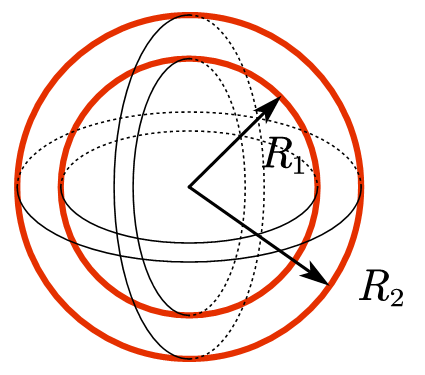
\includegraphics[width=0.5\textwidth]{asset/ch7/T27.png}
        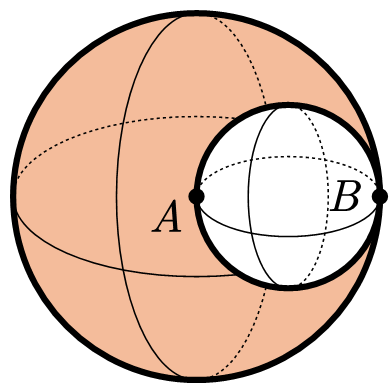
\includegraphics[width=0.45\textwidth]{asset/ch7/T28.png}
    \end{minipage}
    
\end{example}

\begin{example}{利用已知带电体求场强：积分}
    一无限长圆柱面半径为$R$，电荷密度$\sigma=\sigma_0\cos\varphi$（其中$\varphi$为半径与$x$轴的夹角，如下图所示），求圆柱轴线上的场强。
    \tcblower

    根据题意，电荷密度的分布只与$\varphi$有关。若在某处取一窄条（对应圆心角为$d\varphi$），则可视为无限长均匀带电直线，且线电荷密度为$\lambda=\sigma Rd\varphi=\sigma_0 R\cos\varphi d\varphi$

    因为电荷密度的表达式关于$x$轴对称，可以判断场强是$x$方向，只求这一分量即可。

    \vspace{0.5em}

    \begin{minipage}{0.68\linewidth}
     取角度为$\varphi$处的窄条，它在轴线上产生的场强大小为$\dfrac{\sigma_0 R\cos\varphi d\varphi}{2\pi\varepsilon_0 R}$

    在$x$方向上的分量为$-\dfrac{\sigma_0 R\cos^2\varphi d\varphi}{2\pi\varepsilon_0 R}$

    因此整个圆柱面产生的场强为$-\dfrac{\sigma_0}{2\pi\varepsilon_0}\displaystyle\int_0^{2\pi}{ \cos^2\varphi d\varphi}=-\dfrac{\sigma_0}{2\varepsilon_0}$

    这说明场强的大小为$\dfrac{\sigma_0}{2\varepsilon_0}$，方向为$-x$.
    
    \end{minipage}
    \hfill
    \begin{minipage}{0.3\textwidth}
        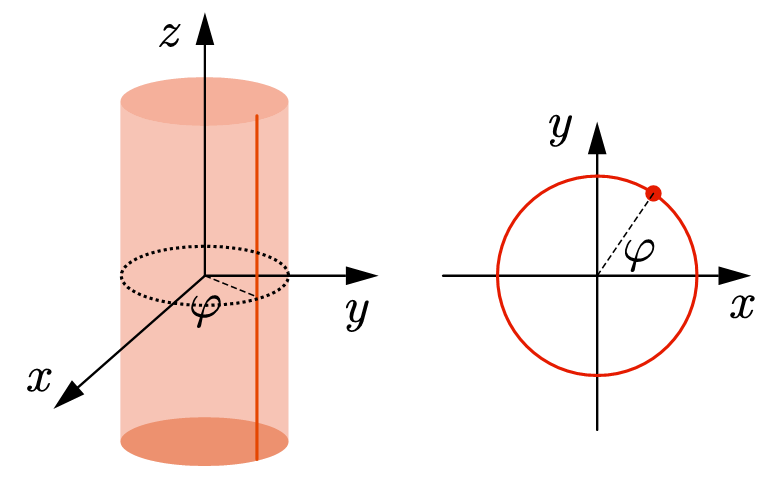
\includegraphics[width=\textwidth]{asset/ch7/T29.png}
    \end{minipage}

    \tcbline
    【补充练习】一个长度无限、宽为$b$的均匀带电平板，电荷面密度为$\sigma=+kx~(0<x<b)$，求薄平板所在平面右侧（$x>b$）的电场分布。
\end{example}

\section{拓展内容}

\subsection{均匀带电直线与圆弧的场强}

\subsubsection{均匀带电圆弧的场强}

\noindent
\begin{minipage}{0.82\linewidth}
\setlength{\parindent}{2em}
\setlength{\parskip}{0.5em}
\linespread{1.3}

对于线电荷密度$\lambda$的均匀带电圆弧，考虑圆心处的场强。

利用对称性，容易判断场强方向一定在圆心角的角平分线上，若圆心角为$2\theta$，可以求出场强大小

\begin{formula}
    $E=\dfrac{2k\lambda}{R}\sin{\theta}$
\end{formula}

\end{minipage}
\hfill
\begin{minipage}{0.15\textwidth}
    
    \centering 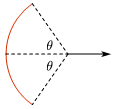
\includegraphics[width=\textwidth]{asset/ch7/T30.png}
\end{minipage}

\subsubsection{均匀带电直线的场强}

均匀带电直线在直线外一点的场强，相当于相同张角的均匀带电圆弧，其半径等于点到直线距离。

\vspace{-1.2em}
\begin{center}
    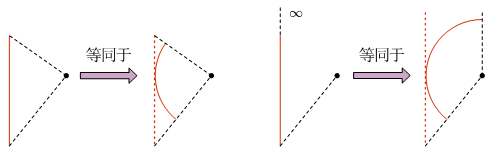
\includegraphics[width=0.6\textwidth]{asset/ch7/T31.png}
\end{center}
\vspace{-1.2em}

\begin{example}{均匀带电直线的场强}
    \begin{minipage}{0.78\linewidth}
     将无限长均匀带电直线弯折成如图所示形状，证明圆心处的场强为零。
    
    \end{minipage}
    \hfill
    \begin{minipage}{0.2\textwidth}
        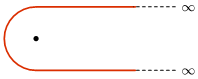
\includegraphics[width=\textwidth]{asset/ch7/T32.png}
    \end{minipage}
    
    \tcblower

    设线电荷密度为$\lambda$，半径为$R$，首先求半圆部分的场强。

    将半圆切分成圆心角$d\theta$的小段，每一段的电荷量$dq=R\lambda d\theta$

    \vspace{0.3em}
    
    在圆心处产生的场强大小为$dE=\dfrac{dq}{4\pi\varepsilon_0 R^2}=\dfrac{\lambda d\theta}{4\pi\varepsilon_0 R}$

    \vspace{0.3em}
    
    以$-x$方向为基准，对于角度为$\theta$的小段，场强的$x$分量大小为$dE_x=\dfrac{\lambda\cos{\theta} d\theta}{4\pi\varepsilon_0 R}$

    \vspace{0.3em}
    
    因此整个半圆的场强大小为$E_1=\displaystyle\int_{-\pi/2}^{\pi/2}\dfrac{\lambda\cos{\theta} d\theta}{4\pi\varepsilon_0 R}=\dfrac{\lambda}{2\pi\varepsilon_0R}$，方向为$+x$

    \vspace{0.3em}
    
    然后求其中一个射线的场强，仍然按照圆心角$d\theta$切小段。

    \vspace{0.3em}

    以$+x$方向为基准，对于角度为$\theta$的小段，$x=\dfrac{R}{\tan\theta}$，两边同时求导得$dx=-\dfrac{Rd\theta}{\sin^2{\theta}}$

    \vspace{0.5em}
    
    所以对于角度为$\theta$的小段，其长度为$dx=\dfrac{Rd\theta}{\sin^2{\theta}}$，电荷量$dq=\dfrac{R\lambda d\theta}{\sin^2{\theta}}$，到圆心距离为$\dfrac{R}{\sin\theta}$

    \vspace{0.3em}
    
    因此它在圆心产生的场强是$dE=\dfrac{dq}{(R/\sin\theta)^2}=\dfrac{\lambda \cdot d\theta}{4\pi\varepsilon_0 R}$，在$x$方向上的分量是$dE_x=\dfrac{\lambda \cos\theta \cdot d\theta}{4\pi\varepsilon_0 R}$

    \vspace{0.5em}
    
    所以一条射线产生的场强的$x$分量为$E_x=\displaystyle\int_0^{\pi/2}\dfrac{\lambda \cos\theta \cdot d\theta}{4\pi\varepsilon_0 R^2}=\dfrac{\lambda}{4\pi\varepsilon_0R}$，方向为$-x$

    \vspace{0.3em}

    根据对称性，另一条射线产生场强的$x$分量也为该值，且$y$分量与之抵消。

    将半圆和射线的$x$分量相加，可得合场强为零。
    
    \tcbline

    \begin{minipage}{0.8\linewidth}
    【补充练习】将无限长均匀带电直线弯折成如图所示形状，线电荷密度为$+\lambda$，求圆心处的场强。
    
    \end{minipage}
    \hfill
    \begin{minipage}{0.18\textwidth}
        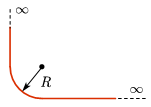
\includegraphics[width=\textwidth]{asset/ch7/T33.png}
    \end{minipage}
\end{example}





\chapter{电势}
\setcounter{example_counter}{1}

\section{电势的概念}

\subsection{静电场的保守性}

\subsubsection{电场力的保守性}

静电力是保守力，这意味着：
\begin{itemize}
    \item 电荷沿任意路径转一圈，静电力做功为零：$\displaystyle \oint_C \vec{F}\cdot d\vec{r}=0$
    \item 电荷从A点到B点，静电力做功与路径无关：$W=\displaystyle\int_{(A)}^{(B)}{\vec{F}\cdot d\vec{r}}$
\end{itemize}

利用$\vec{F}=q\vec{E}$进行变形，即可排除电荷的因素，得到静电场的性质。

\subsubsection{静电场的环路定理}

电场强度沿任意路径转一圈的积分为零，这就是\textbf{静电场的环路定理}。

\begin{formula}
    $\displaystyle \oint_C \vec{E}\cdot d\vec{r}=0$
\end{formula}

\subsection{静电力做功}

\subsubsection{电势差}

电场强度的线积分与路径无关，这一积分结果称为电势差。

A与B的电势差，就等于电场强度沿任意路径从A到B的积分。

\begin{formula}
    $U_{AB}=\varphi_A-\varphi_B=\displaystyle \int_{(A)}^{(B)} \vec{E}\cdot d\vec{r}$
\end{formula}

\warn{注意A与B的电势差，等于A点电势减B点电势，不要减反。}

\subsubsection{电势}

选择任意一点作为电势的零点，即可确定其余各点的电势$\varphi$，习惯上默认取无穷远处为电势零点。

\warn{注意电势是标量，只有大小，没有方向。}

\note{真正有意义的是电势差，电势零点选择不同，各点的电势也不同，但电势差不变。}

\subsubsection{电势能}

因为静电力是保守力，因此可定义电势能，电荷的电势能就等于电荷乘以该点的电势，$E_p=q\varphi$。

根据保守力做功的特点，静电力做功等于电势能的减少量，也等于电荷乘以电势差。

\begin{formula}
    $W=-\Delta E_p=q(\varphi_A-\varphi_B)=qU_{AB}$
\end{formula}

\section{电势的计算}

\subsection{利用电场强度求电势}

某点的电势，就等于电场强度从该点到电势零点的积分。

\begin{formula}
    $\varphi_A=\displaystyle \int_{(A)}^{(0)} \vec{E}\cdot d\vec{r}$
\end{formula}

\begin{example}{利用电场强度求电势}
    有一均匀带电的厚球层，电荷体密度为$\rho$，内外表面半径分别为$R,2R$。(1)~求电场强度的空间分布；(2)~设无穷远处为电势零点，求空腔内任一点的电势。
    \tcblower

    (1)~电荷呈球对称分布，可知场强方向一定沿半径方向，大小可用高斯定理求出，高斯面选择球面。

    当$r<R$时，高斯面内无电荷，$E=0$

    当$R<r<2R$时，高斯面内电荷量为$\dfrac{4}{3}\pi(r^3-R^3)\rho$

    利用高斯定理，$E\cdot 4\pi r^2=\dfrac{4\pi(r^3-R^3)\rho}{3\varepsilon_0}$，得$E=\dfrac{\rho(r^3-R^3)}{3\varepsilon_0 r^2}$

    当$r>2R$时，高斯面内电荷量为$\dfrac{4}{3}\pi[(2R)^3-R^3]\rho=\dfrac{28\pi R^3}{3}\rho$

    利用高斯定理，$E\cdot 4\pi r^2=\dfrac{28\pi R^3\rho}{3\varepsilon_0}$，得$E=\dfrac{7R^3\rho}{3\varepsilon_0 r^2}$

    (2)~球心处的电势为$\varphi=\displaystyle\int_R^{2R}{\dfrac{\rho(r^3-R^3)}{3\varepsilon_0 r^2}dr}+\int_{2R}^{\infty}{\dfrac{7R^3\rho}{3\varepsilon_0 r^2}dr}=\dfrac{3\rho R^2}{2\varepsilon_0}$
    
    \tcbline
    【补充练习】半径为$R,2R$的同轴无限长圆柱面上均匀带电，单位长度的带电量分别为$+\lambda,-\lambda$.~(1)~求电场强度的空间分布；(2)~求内外筒之间的电势差；(3)~以无穷远处为电势零点，求轴线上的电势。
\end{example}

\subsection{电势的叠加原理}

\subsubsection{电势的叠加原理}

一个电荷系的电场中任意一点的电势，等于每个带电体单独存在时在该点产生电势的代数和。

\subsubsection{点电荷的电势}

点电荷周围的电势分布只与到点电荷的距离$r$有关。

\begin{formula}
    $\varphi=\dfrac{q}{4\pi\varepsilon_0r}$
\end{formula}

\note{其实就是$\varphi=\dfrac{kq}{r}$，由此可见，正电荷周围的电势为正，负电荷周围的电势为负。}

\begin{example}{利用叠加原理求电势——离散}
    如图所示，在A、B两点处放有电荷量分别为$+Q,-Q$的点电荷，距离$2R$。(1)~将试探电荷$+q$沿以B为圆心、半径为$R$的半圆从C移动到D，求电场力所做的功；(2)~再将该试探电荷从D移动到无穷远处，求电场力所做的功。
    \tcblower
    
    \tcbline
    【补充练习】边长为$L$的正三角形的三个顶点分别放有电荷量为$+q,~-q,~-2q$的点电荷。(1)~求正三角形中心的电势；(2)~将一个试探电荷$+Q$从无穷远处移动到三角形中心，求电场力所做的功。
\end{example}

\begin{example}{利用叠加原理求电势——连续}
    电荷$+Q$均匀分布在长为$2L$的细杆AB上。(1)~求杆延长线上，到杆端距离为$L$的点C的电势；(2)~质量为$m$、电荷量为$+q$的粒子在静电场中运动，经过点C时的速率为$v$，求该粒子在静电力作用下运动到无穷远处时的速率。
    \tcblower
    
    \tcbline
    【补充练习】真空中有一半径为$R$的半圆细环，均匀带电$+Q$。(1)~以无穷远处为电势零点，求圆心处的电势；(2)~将带电量为$+q$的点电荷从无穷远处移动到圆心，求电场力做的功；(3)~若半圆环不是均匀带电的，圆心处的电场强度和电势会改变吗？
\end{example}

\subsubsection{空心球壳的电势}

对于一个半径为$R$的空心球壳，其外部的电势如同点电荷的电势，内部的电势处处相等。

$\varphi_{\text{外}}=\dfrac{q}{4\pi\varepsilon_0r},~\varphi_{\text{内}}=\dfrac{q}{4\pi\varepsilon_0R}$

\begin{example}{利用已知带电体求电势}
    真空中半径为$R$和$2R$的两个同心球面，其上分别均匀带电$+Q,~-3Q$。(1)~若以无穷远处为电势零点，求两球面之间，到球心距离为$r$的点的电势；(2)~将电荷为$+q$的点电荷紧贴内球面由静止释放，求到达外球面时的动能；(3)~空间中还存在一个零势能面，求其半径。
    \tcblower

    \tcbline
    【补充练习】真空中有一半径为$R$的球面均匀带电，球心处还有一点电荷$+q$，已知球面的电势为$\varphi$。(1)~求球面的电荷量；(2)~求球外任意点的电场强度与电势。
    
\end{example}

\subsection{电势与电场强度的关系}

\subsubsection{等势面}

在电场中电势相等的点组成的曲面称为等势面。

等势面都是闭合的曲面，且与电场线均为垂直相交。

\subsubsection{电势梯度}

若已知电势的空间分布$\varphi(x,y,z)$，则电场强度就是电势梯度的相反数，这是电势下降最快的方向。

\begin{formula}
    $\vec{E}=-\nabla \varphi=-\left(\dfrac{\partial\varphi}{\partial x},\dfrac{\partial\varphi}{\partial y},\dfrac{\partial\varphi}{\partial z}\right)$
\end{formula}

\begin{example}{根据电势求电场强度}
    一半径为$R$的均匀带电细圆环，带电量为$+Q$，水平放置。(1)~求圆环轴线上各点的电势；(2)~求圆环轴线上各点的电场强度；(3)~质量为$m$、电荷量为$+q$的小球，从轴线上方距离圆环$R$的高度静止下落，求运动到圆心时的速率。
    \tcblower
    \tcbline
    【补充练习】半径为$R$的均匀带电圆板，电荷面密度为$+\sigma$.~(1)~求圆盘轴线上各点的电势；(2)~求圆盘轴线上各点的电场强度；(3)~质量为$m$、电荷量为$-q$的粒子，沿轴线从距圆心$R$的位置上向圆心射去，初速度为$v_0$，求击中圆板时的速率。
\end{example}



\section{拓展内容}

\subsection{电偶极子}

相隔一定距离的等量异号点电荷$+q,~-q$，称为\textbf{电偶极子}。

用$\vec{l}$表示从负电荷指向正电荷的矢量线段，则电偶极子的电矩定义为$\vec{p}=q\vec{l}$

电偶极子的电场中所受的合力为零，但合力矩$\vec{M}=\vec{p}\times\vec{E}$

\begin{example}{电偶极子}
    电荷量分别为$+q,-q$的点电荷相距$l$，求其延长线上和中垂线上一点的电场强度。设该点到两电荷中心的距离为$x$，$x\gg l$.
    
    \tcblower
    \tcbline
    【补充练习】两个相同的电偶极子组成一个电四极子，如图所示。求在电四极子延长线上和中垂线上各点的电场强度。

\end{example}

\chapter{电场中的导体与电介质}
\setcounter{example_counter}{1}

\section{电场中的导体}

\subsection{导体的静电平衡条件}

\subsubsection{静电平衡}

导体内部具有自由电子，将导体放在电场中，自由电子将在电场的作用下移动。

导体自由电子的移动，将使导体出现\textbf{感生电荷}，这些电荷也产生电场，与外电场抵消。

当导体内部和表面都没有电荷定向移动时，称为\textbf{静电平衡}。

\subsubsection{静电平衡条件}

处于静电平衡的导体，内部电场为零，表面紧邻处的电场强度与导体表面垂直。

处于静电平衡的导体是等势体，其表面是等势面。

\note{此处所说的电场，应理解为外电场和导体电荷移动所产生电场的叠加。}

\subsubsection{电荷分布}

\begin{itemize}
    \item 处于静电平衡的导体，内部各处净电荷为零，电荷只能分布在表面
    \item 表面各处的面电荷密度，与表面紧邻处的电场强度（合场强）大小成正比
    \item 对于孤立的导体，面电荷密度与表面曲率有关，曲率越大则面电荷密度也越大
\end{itemize}

\note{尖端附近的面电荷密度最大，可产生\textbf{尖端放电}现象。}

利用高斯定理，可求出导体表面附近的电场强度

\begin{formula}
    $E=\dfrac{\sigma}{\varepsilon_0}$
\end{formula}

\warn{注意无限大平板的电场强度大小为$E=\dfrac{\sigma}{2\varepsilon_0}$，不要混淆。}

\subsubsection{静电屏蔽}

金属壳外的电荷在壳内产生的电场为零，即金属壳屏蔽壳外电荷对壳内的影响。

\warn{注意金属壳不能屏蔽壳内电荷对壳外的影响。}

\begin{example}{静电感应}
    (1)~带电量为$+Q$的金属球在P点产生的电场强度大小为$E$，现在P点放一个正试探电荷，它的受力大小等于$qE$吗？如果是负试探电荷呢？(2)~将无限大金属板放在匀强电场$\vec{E}$中，求金属板表面的面电荷密度。
    
    【补充练习】半径为$R$的导体球外部有一电荷$Q$，它到球心的距离为$r>R$。(1)~求球心的场强和电势；(2)~若将导体球接地，求导体球的带电量。
\end{example}

\subsection{有导体存在的电场分析}

\subsubsection{无限大平板}

对于无限大金属平板，无论多薄，都不能忽略其厚度，需要分别设出两个表面的面电荷密度$\sigma$

然后利用每个面的场强为$E=\dfrac{\sigma}{2\varepsilon_0}$和平板内部电场强度为零，利用高斯定理进行求解。

若有某个面接地，则该面上没有电荷，该平板的电势为零。

\begin{example}{无限大导体平板}
    A、B为两个面积$S$足够大的导体平板，平行放置，间距为$d$，分别带电荷$+Q_1,+Q_2$。(1)~求A、B之间的电场强度和电势差；(2)~若将B的下表面接地，求A、B之间的电场强度和电势差。

    【补充练习】三个平行金属板A、B、C的面积都是$S$（足够大），间距分别为$d_1,d_2$，A、C两板接地，B板带电$+Q$。(1)~求各金属板表面的电荷面密度；(2)~求B板的电势。
\end{example}

\subsubsection{导体球与球壳}

若在导体球或球壳外部有电荷，则感应电荷只出现在外表面，球或球壳内部电场强度为零。

若在导体球壳内部有电荷，则感应电荷会出现在内外表面，内表面电荷量与内部电荷抵消，球壳外产生电场。但壳内电荷的位置并不影响外层电荷的分布。

\note{导体球壳的电势公式并不要求电荷是均匀分布的。}

\begin{example}{导体球与球壳}
    内外半径分别为$2R,3R$的导体球壳带有电荷$+Q$，球壳空腔内还有一个点电荷$+Q$，到球心距离为$R$。(1)~求球壳内外表面的电荷，它们的分布均匀吗？(2)~求球心处的电势。

    【补充练习】内外半径分别为$2R,3R$的导体球壳不带电，空腔内还有一个半径为$R$的同心金属球，带电量为$+Q$。(1)~求电荷、电场和电势的分布。(2)~若将球壳接地再断开，求电荷、电场和电势的分布；(3)~若将球壳与金属球用导线相连，求电荷、电场和电势的分布。
\end{example}

\section{电场中的电介质}

\subsection{电介质的电结构特点}

电介质就是通常所说的绝缘体，内部没有可自由移动的电荷。但在电场中，也会因电场的影响，发生电极化现象。

\begin{itemize}
    \item 极性分子在电场中，会发生取向的变化
    \item 非极性分子在电场中，会发生电荷分异
\end{itemize}

在外电场的作用下，电介质表面会束缚电荷（或称为极化电荷），这种现象称为电介质的极化。

\note{导体内部的电荷移动会完全抵消外电场，而电介质的极化只能部分抵消外电场。因此在电介质内部也有电场，但比外电场要弱一些。}

\subsection{电位移}

\subsubsection{电位移矢量}

有电介质存在时，电场分布可用电位移$\vec{D}$描述，单位是$\unit{C/m^2}$。

\begin{formula}
    $\vec{D}=\varepsilon \vec{E}$
\end{formula}

其中，$\varepsilon$表示电介质的介电常数（或电容率），真空的介电常数就是$\varepsilon_0$，因此真空的$\vec{D}=\varepsilon_0 \vec{E}$

介电常数还可以用相对介电常数$\varepsilon_r$描述，表示是真空的多少倍，则$\varepsilon=\varepsilon_0\varepsilon_r$

\note{这一关系仅对各向同性的电介质成立，大学物理课程仅考虑这种电介质。}

\subsubsection{电极化强度}

有电介质存在时，电场是电介质的束缚电荷和其他自由电荷共同产生的，因此电介质与真空的电位移之差，就描述了电介质的极化情况，称为电极化强度$\vec{P}$

\begin{formula}
    $\vec{P}=\vec{D}-\varepsilon_0\vec{E}=\varepsilon_0(\varepsilon_r-1)\vec{E}=\varepsilon_0\chi\vec{E}$
\end{formula}

其中，$\chi=\varepsilon_r-1$也称为电介质的电极化率。

\subsubsection{D的高斯定理}

有电介质存在时，高斯定理仍然成立，即$\displaystyle \varoiint_S {\vec{E}\cdot d\vec{S}}=\dfrac{1}{\varepsilon_0}\sum q_{\text{内}}$，但因为束缚电荷很难知道，所以并不实用。

无论有无电介质存在，通过任意封闭曲面的电位移通量，等于该封闭面包围的自由电荷的代数和，这就是D的高斯定理。

\begin{formula}
    $\displaystyle \varoiint_S {\vec{D}\cdot d\vec{S}}=\sum q_{\text{内自由}}$
\end{formula}

\note{若没有电介质存在，则$\vec{D}=\varepsilon_0 \vec{E}$，就划归为前面所学的高斯定理。}

\warn{注意D的高斯定理只包含内部的自由电荷，不包含束缚电荷。}

\begin{example}{D的高斯定理}
    (1)~若高斯面内不包围自由电荷，则高斯面的下列哪些量为零：(a)~任意点的电场强度；(b)~任意点的电位移矢量；(c)~E通量；(d)~D通量。(2)~若闭合曲面的D通量为零，说明面内电荷情况如何：(a)~没有束缚电荷；(b)~没有自由电荷；(c)~束缚电荷与自由电荷的代数和为零；(d)~自由电荷的代数和为零。
    
    【补充练习】判断以下说法是否正确：(1)~若选择的高斯面通过电介质，则D的高斯定理成立，E的高斯定理不成立；(2)~若高斯面内没有自由电荷，则D通量和E通量均为零；(3)~若高斯面上的电位移矢量处处为零，说明内部自由电荷的代数和为零；(4)~高斯面的D通量仅与内部的自由电荷有关，而E通量与内部和外部的自由电荷都有关。
\end{example}

\begin{example}{有电介质存在的场强}
    一个半径为$R$的薄金属球壳，均匀带电$+Q$。(1)~若球壳内部充满相对介电常数为$\varepsilon_r$的电介质，外部为真空，求电场强度和电势的分布；(2)~若球壳内部为真空，外部包了一层厚度为$R$、相对介电常数为$\varepsilon_r$的电介质，求电场强度和电势的分布。
    \tcblower
    \tcbline
    【补充练习】半径为$R_1,R_2$的无限长同轴金属圆筒，其间充满相对介电常数为$\varepsilon_r$的电介质，设内外圆筒单位长度所带电荷分别为$+\lambda,-\lambda$。求介质中到轴线距离为$r$的电场强度与电位移矢量的大小。
\end{example}

\section{电容}

\subsection{电容器及其电容}

\subsubsection{电容器}

两个彼此绝缘但靠近的导体形成电容器，其电容定义为

\begin{formula}
    $C=\dfrac{Q}{U}$
\end{formula}

\subsubsection{常见的电容器}

电容器的电容可用D的高斯定理求出，一些常见的电容器的电容如下表。

\begin{table}[htb]
    \centering
    \begin{tabular}{|c|c|c|}
        \hline
        电容器的形式 & 图示 & 电容\\
        \hline
        平行板电容器 &  & $C=\dfrac{\varepsilon S}{d}$\\
         \hline
        圆柱形电容器 &  & $C=\dfrac{2\pi \varepsilon L}{\ln{(R_2/R_1)}}$\\
         \hline
        球形电容器 &  & $C=\dfrac{4\pi \varepsilon R_1R_2}{R_2-R_1}$\\
         \hline
        孤立导体球 &  & $C=4\pi\varepsilon R$\\
         \hline
    \end{tabular}
\end{table}

\note{对于一个孤立导体，认为它与无限远处的另一导体组成电容器。}

\subsection{电容器的能量}

电容器的能量储存在电场之中，公式为

\begin{formula}
    $W=\dfrac{1}{2}QU=\dfrac{1}{2}CU^2=\dfrac{1}{2}\cdot\dfrac{Q^2}{C}$
\end{formula}

\begin{example}{电容器}
    内外半径分别为$R_1,R_2$的圆柱形电容器，间隙填满相对介电常数为$\varepsilon_r$的电介质，若电容内的电场强度最大不能超过$E_m$，求达到极限时的电压、电荷量、储存的电能。
    
    【补充练习】内外半径分别为$R_1,R_2$的同心球形电容器，间隙填满相对介电常数为$\varepsilon_r$的电介质。当内外球面带电量为$Q$时，求：(1)~内外球面的电势差；(2)~电场强度的分布；(3)~储存的电能。
\end{example}

\begin{example}{电容的动态分析}
    一平行板电容器，极板之间为真空，极板间距为$d$，面积为$S$，充电后切断电源。分别进行以下操作，判断电容、带电量、电场强度、电压、电场能量如何变化。(1)~将极板间距变为$2d$；(2)~将极板错开，使相对面积变为$S/2$；(3)~插入一块厚度为$d/2$的金属导体；(4)~填满相对介电常数为$\varepsilon_r$的电介质。
    \tcblower
    \tcbline
    【补充练习】一平行板电容器，极板之间为真空，极板间距为$d$，面积为$S$，始终与直流电源相连。分别进行以下操作，判断电容、带电量、电场强度、电压、电场能量如何变化。(1)~将极板间距变为$2d$；(2)~将极板错开，使相对面积变为$S/2$；(3)~插入一块厚度为$d/2$的金属导体；(4)~填满相对介电常数为$\varepsilon_r$的电介质。
    
\end{example}

\subsection{电容的串并联}

\begin{itemize}
    \item 几个电容并联，总电容等于各个电容之和
    \item 几个电容串联，总电容的倒数等于各个电容的倒数和
\end{itemize}

\begin{formula}
    $C_{\text{并}}=\sum{C_i},~\dfrac{1}{C_{\text{串}}}=\sum{\dfrac{1}{C_i}}$
\end{formula}

\note{电容串并联规律与电阻是相反的，与弹簧是相同的。}



\section{拓展内容}

\subsection{唯一性定理与镜像法}



\subsection{静电场的边界条件}

\subsection{电场的能量}

\subsubsection{电荷系的能量}

对于多个电荷组成的系统，把各个电荷从无穷远聚集到现在位置，克服电场力所做的功，称为电荷系的静电能。静电能也可以定义为，将各电荷从现有位置分散到无穷远，静电力所做的功。

\begin{formula}
    离散：$W=\dfrac{1}{2}\sum{q_i\varphi_i}$~~~连续：$W=\dfrac{1}{2}\displaystyle\int_q{\varphi dq}$
\end{formula}

其中，$\varphi_i$表示除$q_i$外的其他电荷在$q_i$处产生的电势。

\subsubsection{电场的能量}

电场在单位体积内的能量称为能量密度$w$，电场的总能量$W$就是全空间上能量密度的体积分。

\begin{formula}
    $w=\dfrac{1}{2}\vec{D}\cdot\vec{E}=\dfrac{1}{2}\varepsilon E^2,~~W=\displaystyle\iiint_V wdV$
\end{formula}

\begin{example}{电场的能量}
    有一橡胶做的气球，可视为半径为$R$的球面，电荷$+Q$在上面均匀分布。(1)~求电场的能量；(2)~若电荷量变为原来的2倍，电场能量如何变化？(3)~若电荷量不变，但将其吹大，半径从$R$变为$2R$，则电场能量如何变化？
    
    【补充练习】地球表面上空晴天时的电场强度约为$\SI{100}{V/m}$。(1)~求电场的能量密度；(2)~若整个地球表面以上$\SI{10}{km}$范围内电场强度都是这一数值，取地球半径为$\SI{6400}{km}$，求这一范围内的电场能。
\end{example}

\subsection{电容的串并联分析}

\begin{example}{电容的串并联}
    如图所示，空气电容器$C_1=\SI{10}{\mu F},C_2=C_3=\SI{5}{\mu F}$。(1)~求总电容；(2)~若连接$\SI{100}{V}$直流电源充电，求各电容的电荷量和电压；(3)~若保持连接直流电源，将一电介质插入$C_1$中，各电容器的电压如何变化？(4)~若将电源断开，再将一电介质插入$C_1$中，各电容器的电压如何变化？
    
    【补充练习】一平行板电容器，极板之间为真空，极板间距为$d$，面积为$S$，充电后切断电源。在其中插入一块电介质，两极板的电压变为原来的一半，在以下两种情况下求相对介电常数，并求出自由电荷与极化电荷的分布。(1)~电介质的面积也为$S$，厚度为$d/3$；(2)~电介质的厚度为$d$，但面积为$S/3$.
\end{example}

%\chapter{稳恒电流的磁场}
\setcounter{example_counter}{1}

\section{电流与电动势}

\subsection{电流}

\subsubsection{电流强度}

电流是电荷的定向运动，单位时间内通过某一截面的电量称为电流强度，简称电流。

\begin{formula}
    $I=\dfrac{dq}{dt}$
\end{formula}

电流强度是标量，只有大小，没有方向。

\subsubsection{电流密度}

电流密度矢量$\vec{j}$能同时描述各处电流的大小和方向，它的方向就是正电荷运动的方向，大小等于通过该点单位面积的电流密度。

\begin{formula}
    $dI=\vec{j}\cdot d\vec{S}~~~I=\displaystyle \iint_S{\vec{j}\cdot d\vec{S}}$
\end{formula}

\subsection{电动势}

电源的电动势$\mathcal E$，是电源把单位正电荷从负极移向正极过程中，非静电力所做的功。

单位正电荷受到的非静电力，称为“非静电场的场强”，则电动势就是这种场强沿闭合回路的积分。

\begin{formula}
    $\mathcal E=\dfrac{W_{\text{非}}}{q}=\displaystyle\oint_L{\vec{E}_{\text{非}}\cdot d\vec{l}}$
\end{formula}

\section{恒定电流产生的磁场}

\subsection{毕奥-萨伐尔定律}

载有电流的长度为$dl$的通电导线，称为一个电流元，用$Id\vec{l}$表示，方向与电流方向相同。

对于电流元$Id\vec{l}$，用$\vec{r}$表示它指向P点的向量，则电流元在P点产生的磁场为

\begin{formula}
    $d\vec{B}=\dfrac{\mu_0}{4\pi}\dfrac{Id\vec{l}\times\vec{e}_r}{r^2}$
\end{formula}

其中，$\mu_0$称为真空磁导率，$\mu_0=\dfrac{1}{\varepsilon_0c^2}=4\pi\times10^{-7}\unit{N/A^2}$

若记电流元$Id\vec{l}$与$\vec{r}$的夹角为$\theta$，则磁场强度的大小为$\dfrac{\mu_0}{4\pi}\dfrac{Id\vec{l}\sin{\theta}}{r^2}$，方向垂直于二者所确定的平面。

\note{在电流元延长线上的点，电流元不产生磁场。}

\subsection{磁通连续定理（磁场的高斯定理）}

目前并未发现单独存在的磁单极子，磁场是无源有旋场，在任何磁场中，通过任意封闭曲面的磁通量都为零。

\begin{formula}
    $\displaystyle\varoiint_S{\vec{B}}\cdot d\vec{S}=0$
\end{formula}

\subsection{典型电流的磁场分布}

\section{安培环路定理}

\subsection{安培环路定理}

在恒定电流的磁场中，磁感应强度沿任何路径的线积分，等于路径包围电流强度之和的$\mu_0$倍。

\begin{formula}
    $\displaystyle\oint_C {\vec{B}\cdot d\vec{c}}=\mu_0 \sum{I_{\text{内}}}$
\end{formula}

\subsection{利用安培环路定理求磁场分布}

\section{拓展内容}

\subsection{电流的微观解释}

\subsection{基尔霍夫定律}

\subsection{运动电荷产生的磁场}

电流是电荷运动产生的，因此运动的电荷也可产生磁场，计算方法与毕奥-萨伐尔定律相似。

\begin{formula}
    $d\vec{B}=\dfrac{\mu_0}{4\pi}\dfrac{q\vec{v}\times\vec{e}_r}{r^2}$
\end{formula}



\chapter{稳恒电流的磁场}
\setcounter{example_counter}{1}

\section{电流与电动势}

\subsection{电流}

\subsubsection{电流强度}

电流是电荷的定向运动，单位时间内通过某一截面的电量称为电流强度，简称电流。

\begin{formula}
    $I=\dfrac{dq}{dt}$
\end{formula}

电流强度是标量，只有大小，没有方向。

\subsubsection{电流密度}

电流密度矢量$\vec{j}$能同时描述各处电流的大小和方向，它的方向就是正电荷运动的方向，大小等于通过该点单位面积的电流密度。

\begin{formula}
    $dI=\vec{j}\cdot d\vec{S}~~~I=\displaystyle \iint_S{\vec{j}\cdot d\vec{S}}$
\end{formula}

\note{电流密度与电流强度的关系：$I=\displaystyle\iint_S\vec{j}\cdot d\vec{S}$，即通过某一截面的电流等于电流密度矢量对该截面通量。}

\begin{example}{电流密度的计算}
    有一根半径为$R$的均匀导线，电流为$I$均匀通过导线截面。求导线内部距离轴线为$r$处的电流密度大小。
    \tcblower
    电流均匀通过导线截面，说明电流密度方向沿轴线方向，大小处处相等。

    对于距离轴线为$r$处的圆面，其面积为$\pi r^2$，通过该面积的电流为

    $I=\dfrac{\pi r^2}{\pi R^2}\cdot I=\dfrac{r^2}{R^2}I$

    根据电流密度的定义，$j=\dfrac{I}{S}$，因此

    $j=\dfrac{I}{\pi r^2}\cdot\dfrac{r^2}{R^2}=\dfrac{I}{\pi R^2}$

    可知均匀导线中电流密度大小处处相等，方向沿轴线方向。

    \tcbline
    【补充练习】若电流在导线截面上不是均匀分布，而是满足$j=j_0(1-\dfrac{r}{R})$，其中$j_0$为轴线处的电流密度，$r$为到轴线的距离，求通过导线截面的总电流。
\end{example}

\subsection{电动势}

电源的电动势$\mathcal E$，是电源把单位正电荷从负极移向正极过程中，非静电力所做的功。

单位正电荷受到的非静电力，称为“非静电场的场强”，则电动势就是这种场强沿闭合回路的积分。

\begin{formula}
    $\mathcal E=\dfrac{W_{\text{非}}}{q}=\displaystyle\oint_L{\vec{E}_{\text{非}}\cdot d\vec{l}}$
\end{formula}

\note{电动势与端电压的区别：电动势是电源本身的性质，取决于电源把单位正电荷从负极移到正极时非静电力所做的功；而端电压是电源两极之间的电势差，当电路断开时，端电压等于电动势；当电路接通时，端电压小于电动势（因为电源有内阻）。}

\section{恒定电流产生的磁场}

\subsection{毕奥-萨伐尔定律}

载有电流的长度为$dl$的通电导线，称为一个电流元，用$Id\vec{l}$表示，方向与电流方向相同。

对于电流元$Id\vec{l}$，用$\vec{r}$表示它指向P点的向量，则电流元在P点产生的磁场为

\begin{formula}
    $d\vec{B}=\dfrac{\mu_0}{4\pi}\dfrac{Id\vec{l}\times\vec{e}_r}{r^2}$
\end{formula}

其中，$\mu_0$称为真空磁导率，$\mu_0=\dfrac{1}{\varepsilon_0c^2}=4\pi\times10^{-7}\unit{N/A^2}$

若记电流元$Id\vec{l}$与$\vec{r}$的夹角为$\theta$，则磁场强度的大小为$\dfrac{\mu_0}{4\pi}\dfrac{Id\vec{l}\sin{\theta}}{r^2}$，方向垂直于二者所确定的平面。

\note{在电流元延长线上的点，电流元不产生磁场。}

\subsection{磁通连续定理（磁场的高斯定理）}

目前并未发现单独存在的磁单极子，磁场是无源有旋场，在任何磁场中，通过任意封闭曲面的磁通量都为零。

\begin{formula}
    $\displaystyle\varoiint_S{\vec{B}}\cdot d\vec{S}=0$
\end{formula}

\subsection{典型电流的磁场分布}

与第7章中典型带电体的电场分布类似，本节讨论几种典型电流分布产生的磁场。

\subsubsection{载流直导线}

设有一根无限长直导线载有电流$I$，求距导线为$a$处的磁感应强度。

取电流元$Id\vec{l}$，设它到P点的距离为$r$，电流元与$\vec{r}$的夹角为$\theta$。则电流元在P点产生的磁场大小为$dB=\dfrac{\mu_0}{4\pi}\dfrac{Idl\sin\theta}{r^2}$，方向由右手定则确定。

\begin{example}{无限长直导线周围的磁场}
    求无限长直导线外距离导线$a$处的磁感应强度。
    \tcblower
    建立如图所示坐标系，设P点到导线的垂足为O，$OP=a$，电流元$Id\vec{l}$到P点的连线与电流方向的夹角为$\theta$。

    设电流元到O点的距离为$l$，则$r=\sqrt{l^2+a^2}$，$\sin\theta=\dfrac{a}{\sqrt{l^2+a^2}}$

    因此$dB=\dfrac{\mu_0}{4\pi}\dfrac{Idl\cdot a}{(l^2+a^2)^{3/2}}$

    积分范围从$-\infty$到$+\infty$，可得

    \vspace{0.5em}

    $B=\displaystyle\int_{-\infty}^{+\infty}{\dfrac{\mu_0}{4\pi}\dfrac{Ia\,dl}{(l^2+a^2)^{3/2}}}=\dfrac{\mu_0 I}{2\pi a}$

    \vspace{0.5em}

    方向由右手定则确定：若电流向上，则磁场方向为逆时针（俯视）；若电流向下，则磁场方向为顺时针。

    \tcbline
    【补充练习】两根无限长直导线相互平行，电流分别为$I_1$和$I_2$，方向相同，距离为$d$。求两根导线之间的作用力。
\end{example}

\note{无限长直导线周围的磁场大小与距离成反比，$B=\dfrac{\mu_0 I}{2\pi r}$，方向沿切线方向。}

\subsubsection{载流圆线圈}

设有一半径为$R$的载流圆线圈，电流为$I$，求圆心处的磁感应强度。

对于圆线圈上的任一电流元$Id\vec{l}$，它到圆心的连线与电流方向的夹角为$90^\circ$，因此在圆心处产生的磁场大小为$dB=\dfrac{\mu_0}{4\pi}\dfrac{Idl}{R^2}$，方向沿轴线方向。

\begin{example}{圆电流中心的磁场}
    求载流圆线圈在圆心处的磁感应强度。
    \tcblower
    对于圆线圈上的任意电流元$Id\vec{l}$，电流方向与到圆心连线的夹角均为$90^\circ$，因此在圆心处产生的磁场大小为

    $dB=\dfrac{\mu_0}{4\pi}\dfrac{Idl\sin90^\circ}{R^2}=\dfrac{\mu_0}{4\pi}\dfrac{Idl}{R^2}$

    整个圆线圈积分可得

    $B=\displaystyle\int_0^{2\pi R}{\dfrac{\mu_0}{4\pi}\dfrac{Idl}{R^2}}=\dfrac{\mu_0 I}{2R}$

    方向由右手定则确定：若电流为逆时针（俯视），则磁场方向垂直于线圈平面向外；若电流为顺时针，则磁场方向垂直于线圈平面向里。

    \tcbline
    【补充练习】一半径为$R$的圆形线圈，电流为$I$。求在线圈轴线上距离圆心为$x$处的磁感应强度。
\end{example}

\note{圆电流中心的磁场大小为$B=\dfrac{\mu_0 I}{2R}$，方向由右手定则确定。}

\subsubsection{载流螺线管}

螺线管是由密绕的载流导线组成的螺旋管。若螺线管的长度远大于其半径，可视为无限长螺线管。

\begin{example}{长直螺线管内部的磁场}
    设长直螺线管的半径为$R$，单位长度匝数为$n$，电流为$I$。求螺线管内部的磁感应强度。
    \tcblower
    对于无限长螺线管，可判断其磁场具有轴对称性：
    \begin{itemize}
        \item 螺线管内部为匀强磁场，方向沿轴线方向
        \item 螺线管外部磁场近似为零
    \end{itemize}

    取安培环路为矩形回路$abcd$，其中$ab$边平行于轴线，位于螺线管内部，长度为$l$；$cd$边在螺线管外；$bc$和$da$边垂直于轴线。

    根据安培环路定理：
    \begin{itemize}
        \item 在$ab$边上，$\vec{B}$与$d\vec{l}$方向相同，$\vec{B}\cdot d\vec{l}=B\,dl$
        \item 在$cd$边上，$B\approx0$
        \item 在$bc$和$da$边上，$\vec{B}$与$d\vec{l}$垂直
    \end{itemize}

    因此$\displaystyle\oint\vec{B}\cdot d\vec{l}=Bl$

    环路包围的电流为$nIl$，根据安培环路定理：

    $Bl=\mu_0 nIl$

    得$B=\mu_0 nI$

    \tcbline
    【补充练习】有一匝数为$N$、半径为$R$、长度为$L$的螺绕环，电流为$I$。求环内磁感应强度的分布。
\end{example}

\note{长直螺线管内部为匀强磁场，$B=\mu_0 nI$，方向由右手定则确定（用右手握住螺线管，四指指向电流方向，则拇指指向磁场方向）。}

\subsubsection{环形螺线管（螺绕环）}

环形螺线管即螺绕环，是绕在环形管上的线圈。

\begin{formula}
    $B=\dfrac{\mu_0 NI}{2\pi r}$
\end{formula}

其中$N$为总匝数，$r$为环内一点到环心的距离。当环的半径远大于横截面半径时，环内磁场可近似为匀强。

\note{螺绕环是磁场的"环形螺线管"，其磁场主要分布在环内，$B=\dfrac{\mu_0 NI}{2\pi r}$。}

\section{安培环路定理}

\subsection{安培环路定理}

在恒定电流的磁场中，磁感应强度沿任何路径的线积分，等于路径包围电流强度之和的$\mu_0$倍。

\begin{formula}
    $\displaystyle\oint_C {\vec{B}\cdot d\vec{c}}=\mu_0 \sum{I_{\text{内}}}$
\end{formula}

\subsection{利用安培环路定理求磁场分布}

虽然安培环路定理适用于任何电流分布的磁场，但利用安培环路定理求磁感应强度时，只能解决具有对称性的情况。

与高斯定理类似，使用安培环路定理求解磁场的条件是：磁场的分布必须具有某种对称性，使得$\vec{B}$的大小在积分回路上容易判断，且$\vec{B}$的方向与回路切线方向夹角要么为$0^\circ$要么为$90^\circ$。

常见具有对称性的电流分布包括：无限长直导线、无限长螺线管、环形螺线管等。

\begin{example}{利用安培环路定理求无限长直导线的磁场}
    利用安培环路定理求无限长直导线周围的磁场分布。
    \tcblower
    首先分析磁场的对称性：
    \begin{itemize}
        \item 无限长直导线的磁场具有轴对称性
        \item 磁场方向沿切线方向（由右手定则确定）
        \item 磁场大小只与到导线的距离有关
    \end{itemize}

    取安培环路为以导线为圆心、半径为$r$的圆周$C$，方向与电流方向满足右手定则。

    在圆周上，$\vec{B}$的大小处处相等，方向与$d\vec{l}$方向相同，因此

    $\displaystyle\oint_C\vec{B}\cdot d\vec{l}=B\cdot 2\pi r$

    环路包围的电流为$I$，根据安培环路定理：

    $B\cdot 2\pi r=\mu_0 I$

    得$B=\dfrac{\mu_0 I}{2\pi r}$

    \tcbline
    【补充练习】有一根无限长直圆筒导体，电流$I$均匀分布在圆筒的截面上。求圆筒内部（$r<R$）和外部（$r>R$）的磁场分布。
\end{example}

\begin{example}{利用安培环路定理求无限长螺线管的磁场}
    利用安培环路定理求无限长螺线管内部的磁场分布。
    \tcblower
    首先分析磁场的对称性：
    \begin{itemize}
        \item 无限长螺线管的磁场具有轴对称性
        \item 螺线管内部为匀强磁场，方向沿轴线方向
        \item 螺线管外部磁场近似为零
    \end{itemize}

    取安培环路为矩形回路$abcd$，其中$ab$边平行于轴线，长度为$l$，位于螺线管内部。

    在$ab$边上，$\vec{B}$与$d\vec{l}$方向相同；在$cd$边上，$B\approx0$；在$bc$和$da$边上，$\vec{B}$与$d\vec{l}$垂直。

    因此$\displaystyle\oint\vec{B}\cdot d\vec{l}=Bl$

    环路包围的电流为$nIl$（$n$为单位长度匝数），根据安培环路定理：

    $Bl=\mu_0 nIl$

    得$B=\mu_0 nI$

    \tcbline
    【补充练习】若螺线管不是无限长，但长度$L$远大于半径$R$，求螺线管内部靠近中心处的磁场大小。
\end{example}

\begin{example}{利用安培环路定理求螺绕环的磁场}
    利用安培环路定理求螺绕环内部的磁场分布。
    \tcblower
    首先分析磁场的对称性：
    \begin{itemize}
        \item 螺绕环的磁场具有轴对称性
        \item 磁场方向沿环的切线方向（环绕环轴）
        \item 磁场大小只与到环心的距离有关
    \end{itemize}

    取安培环路为以环心为圆心、半径为$r$的圆周$C$（$r$在环内）。

    在圆周上，$\vec{B}$的大小处处相等，方向与$d\vec{l}$方向相同，因此

    $\displaystyle\oint_C\vec{B}\cdot d\vec{l}=B\cdot 2\pi r$

    环路包围的电流为$NI$（$N$为总匝数），根据安培环路定理：

    $B\cdot 2\pi r=\mu_0 NI$

    得$B=\dfrac{\mu_0 NI}{2\pi r}$

    \note{当环的半径远大于横截面半径时，可近似认为环内磁场均匀，$B\approx\dfrac{\mu_0 NI}{2\pi R}$，其中$R$为环的平均半径。}

    \tcbline
    【补充练习】有一根同轴电缆，内芯半径为$R_1$，外皮半径为$R_2$，电流$I$从内芯流入，从外皮流出。求各区域的磁场分布。
\end{example}

\note{使用安培环路定理的关键在于：1）分析磁场对称性；2）选择合适的安培环路（通常是与磁场方向平行的直线或与磁场方向垂直的圆）；3）判断环路包围的电流。}

\section{拓展内容}

\subsection{电流的微观解释}

从微观角度来看，电流是大量带电粒子的定向运动。设导体单位体积内的自由电荷数为$n$，每个电荷的电荷量为$q$，定向运动的平均速度为$v$（称为漂移速度），导体的横截面积为$S$，则电流强度为

\begin{formula}
    $I=nqSv$
\end{formula}

相应地，电流密度矢量为

\begin{formula}
    $\vec{j}=nq\vec{v}$
\end{formula}

\note{漂移速度$v$通常非常小（数量级约为$10^{-4}\unit{m/s}$），但由于单位体积内的自由电荷数$n$非常大，因此可以形成可观的电流。}

\begin{example}{金属导线的电流}
    有一根铜导线，横截面积为$\SI{1}{mm^2}$，电流为$\SI{1}{A}$。已知铜的自由电子密度为$n=\SI{8.5e28}{m^{-3}}$，电子电荷量为$e=\SI{1.6e-19}{C}$。求自由电子的漂移速度。
    \tcblower
    根据$I=nqvS$，漂移速度

    $v=\dfrac{I}{nqS}=\dfrac{1}{8.5\times10^{28}\times1.6\times10^{-19}\times10^{-6}}=\SI{7.4e-5}{m/s}$

    可以看到，漂移速度是非常小的，这也说明了电流的传播速度（实际上是电场的传播速度）远大于电荷的定向运动速度。

    \tcbline
    【补充练习】若要使漂移速度达到$\SI{1}{mm/s}$，则需要多大的电流？（假设导线参数不变）
\end{example}

\subsection{基尔霍夫定律}

基尔霍夫定律是电路分析的基本定律，包括电流环路定理和电压环路定理。

\subsubsection{基尔霍夫电流定律（KCL）}

基尔霍夫电流定律指出：对于电路中的任意节点，流入节点的电流代数和等于流出节点的电流代数和。

\begin{formula}
    $\displaystyle\sum I_{\text{入}}=\sum I_{\text{出}}$
\end{formula}

这一定律的本质是电荷守恒，因为在稳恒电流中，电荷不会在节点处累积。

\note{基尔霍夫电流定律不仅适用于节点，也适用于任意闭合区域。}

\subsubsection{基尔霍夫电压定律（KVL）}

基尔霍夫电压定律指出：对于电路中的任意回路，沿回路绕行一周，各段电压的代数和为零。

\begin{formula}
    $\displaystyle\sum U=0$
\end{formula}

这一定律的本质是能量守恒，因为单位正电荷沿闭合回路一周回到原点，电势能不变。

\begin{example}{利用基尔霍夫定律解电路}
    有一个回路如图所示，电源电动势分别为$\mathcal E_1=\SI{12}{V}$、$\mathcal E_2=\SI{6}{V}$，内阻分别为$r_1=\SI{1}{\Omega}$、$r_2=\SI{0.5}{\Omega}$，外电阻$R_1=\SI{5}{\Omega}$、$R_2=\SI{4}{\Omega}$。求各支路的电流。
    \tcblower
    设电流$I_1$和$I_2$如图所示，对回路应用基尔霍夫电压定律：

    $\mathcal E_1-\mathcal E_2=I_1(r_1+R_1)-I_2(R_2+r_2)$

    解得$I_1=\SI{1.5}{A}$，$I_2=\SI{0.75}{A}$

    \tcbline
    【补充练习】若在两电源之间再并联一个电阻$R_3=\SI{10}{\Omega}$，求各支路的电流。
\end{example}

\note{基尔霍夫定律是第7章回路定理的推广，可作为复习。}

\subsection{运动电荷产生的磁场}

电流是电荷运动产生的，因此运动的电荷也可产生磁场，计算方法与毕奥-萨伐尔定律相似。

\begin{formula}
    $d\vec{B}=\dfrac{\mu_0}{4\pi}\dfrac{q\vec{v}\times\vec{e}_r}{r^2}$
\end{formula}



\chapter{磁力与磁介质}
\setcounter{example_counter}{1}

\section{磁力}

\subsection{安培力}

\subsection{洛伦兹力}

\subsection{霍尔效应}

\section{磁介质}

\section{拓展内容}

\chapter{电磁感应}
\setcounter{example_counter}{1}

\section{法拉第电磁感应定律}

\section{互感与自感}

\section{磁场的能量}

\section{麦克斯韦方程组}

\colorlet{maincolor}{Black}
\colorlet{sidecolor}{Black!50}

\silentpart{附录~~补充练习答案}

\chapter*{补充练习答案}

\section*{第7章}

\noindent 1.~~~原带电体可以看做两个部分的叠加：

(1)~八个顶点均为$q=\SI{1e-6}{C}$电荷的立方体，根据对称性，这在正方体中心处的电场强度为零

(2)~在一个顶点处$-2q$的点电荷，这个点电荷到正方体中心的距离是体对角线的一半，即$\dfrac{\sqrt{3}}{2}L$.

因此场强的大小为$E=\dfrac{2q}{4\pi\varepsilon_0 (\sqrt{3}L/2)^2}=\SI{2.4e4}{V/m}$，方向指向负电荷。

\noindent\hdashrule{\textwidth}{1pt}{1pt}

\noindent 2.~~~(1)~根据对称性，只需求$y$分量。

将半圆切分成圆心角为$d\theta$的小段，每段长度为$Rd\theta$，带电量为$dq=2Q\dfrac{Rd\theta}{\pi R}=\dfrac{2Qd\theta}{\pi}$

每个小段产生的电场强度大小为$dE=\dfrac{dq}{4\pi\varepsilon_0 R^2}=\dfrac{Qd\theta}{2\pi^2\varepsilon_0 R^2}$

对于角度为$\theta$的小段，其$y$分量的大小为$dE_y=\dfrac{Q\sin{\theta}d\theta}{2\pi^2\varepsilon_0 R^2}$，方向为$-y$

因此整个细线产生的场强大小为$\displaystyle \int_0^\pi {\dfrac{Q\sin{\theta}d\theta}{2\pi^2\varepsilon_0 R^2}}=-\left.\dfrac{Q\cos{\theta}}{2\pi^2\varepsilon_0 R^2}\right|_0^\pi=\dfrac{Q}{\pi^2\varepsilon_0 R^2}$，方向为$-y$

(2)~根据对称性，只需求$x$分量，$y$分量可相互抵消。

对于右半部分，场强大小与上一问相同，$x$分量的大小为$dE_x=\dfrac{Q\cos{\theta}d\theta}{2\pi^2\varepsilon_0 R^2}$，方向为$+x$

因此右半部分产生的场强的$x$分量为$dE_x=\displaystyle \int_0^{\pi/2}\dfrac{Q\cos{\theta}d\theta}{2\pi^2\varepsilon_0 R^2}=\left.\dfrac{Q\sin{\theta}}{2\pi^2\varepsilon_0 R^2}\right|_0^{\pi/2}=\dfrac{Q}{2\pi^2\varepsilon_0 R^2}$

同理，左半部分产生场强的$x$分量也为此值，且方向也为$+x$

因此整个细线产生的场强大小为$\dfrac{Q}{\pi^2\varepsilon_0 R^2}$，方向为$+x$

\noindent\hdashrule{\textwidth}{1pt}{1pt}

\noindent 3.~~~将半球面沿轴线切分成若干圆心角为$d\theta$的圆环

每个圆环宽度为$Rd\theta$，折合线电荷密度为$\lambda=\sigma Rd\theta$

则对于角度为$\theta$的圆环，其半径为$R\sin{\theta}$，周长为$2\pi R\sin{\theta}$

乘以宽度得到面积$2\pi R^2\sin{\theta}d\theta$，其带电量为$2\pi R^2\sigma \sin{\theta}d\theta$

球心到这个圆环所在平面的距离$x=R\sin\theta$，例3已求出环形细线在各点处的场强

利用该结果可得这个圆环在圆心产生的场强是$dE=\dfrac{R\cos\theta \cdot \sigma Rd\theta\cdot R\sin\theta}{2\varepsilon_0 R^3}=\dfrac{\sigma\sin2\theta d\theta }{4\varepsilon_0}$ 

整个半球面的场强为$E=\displaystyle\int_0^{\pi/2}{\dfrac{\sigma\sin2\theta d\theta}{4\varepsilon_0}}=-\left.\dfrac{\sigma\cos 2\theta}{8\varepsilon_0}\right|_0^{\pi/2}=\dfrac{\sigma}{4\varepsilon_0}$，方向沿轴线远离半球面

\newpage

\noindent 4.~~~假想作出一个以电荷为球心，$\sqrt{2}R$为半径的球

则点电荷发出的电场线，能通过要求平面的，都能穿过该平面所截得的球冠，且均为垂直穿过。

利用球冠面积公式，可得$S=2\pi \sqrt{2}R (\sqrt{2}R-R)=2(2-\sqrt{2})\pi R^2$

在该球上各点的电场强度大小均为$E=\dfrac{q}{4\pi\varepsilon_0 (\sqrt{2}R)^2}=\dfrac{q}{8\pi\varepsilon_0 R^2}$
，电通量$\Phi_e=E\cdot S=\dfrac{(2-\sqrt{2}) q}{4\varepsilon_0}$

\noindent\hdashrule{\textwidth}{1pt}{1pt}

\noindent 5.~~~(1)~错误，高斯定理适用于所有的静电场，但只能用于求具有对称性的电场强度。

(2)~错误，外部电荷不影响电通量，但会影响场强，所以场强可以不为零。

(3)~错误，高斯面上场强处处为零，说明电通量为零，但只能说明内部净电荷为零，可能正负抵消。

(4)~错误，场强处处不为零，但电通量可能为零，内部可以无电荷。

(5)~正确，根据高斯定理，电通量与内部净电荷成正比。

\noindent\hdashrule{\textwidth}{1pt}{1pt}

\noindent 6.~~~(1)~电场线为$+x$方向，因此只需关注与之垂直的两个面。

电场线从$x=1$处穿入，从$x=2$处穿出，两处场强大小分别为$E_1=800~\unit{V/m},~E_2=800\sqrt{2}~\unit{V/m}$

若以从内到外穿出为正，则通过立方体的电通量为$\Phi_e=E_2 S- E_1 S=800(\sqrt{2}-1)~\unit{V\cdot m}$

(2)~根据高斯定理，$\Phi_e=\dfrac{\sum q_{\text{内}}}{\varepsilon_0}$，得内部总电荷量$\sum q_{\text{内}}=\Phi_e \varepsilon_0\approx \SI{2.9E-9}{C}$，且为正电荷。

\noindent\hdashrule{\textwidth}{1pt}{1pt}

\noindent 7.~~~(1)~这是一个柱对称的带电体，可知电场线全部沿半径方向指向外侧。

取高斯面为圆柱面，半径为$r$，高为$H$，则由高斯定理，$\Phi_e=\dfrac{\sum q_{\text{内}}}{\varepsilon_0}=2\pi rH\cdot E$，即$E=\dfrac{\sum q_{\text{内}}}{2\varepsilon_0\pi rH}$

\begin{itemize}
    \item 当$r<R$时，高斯面内无电荷，$\sum q_{\text{内}}=0$，因此$E=0$
    \item 当$R\leq r<2R$时，$\sum q_{\text{内}}=\rho\pi(r^2-R^2)H$，得$E=\dfrac{\rho(r^2-R^2)}{2\varepsilon_0 r}$
    \item 当$r\geq 2R$时，$\sum q_{\text{内}}=\rho\pi[(2R)^2-R^2]H=3\rho\pi R^2 H$，得$E=\dfrac{3\rho R^2}{2\varepsilon_0 r}$
\end{itemize}

(2)~这是一个面对称的带电体，以厚壁中心为对称面，电场线全部垂直对称面指向外侧。

取高斯面为柱面，底面积为$S$，且底面与对称面平行，位于坐标为$\pm x$处。

由高斯定理，$\Phi_e=\dfrac{\sum q_{\text{内}}}{\varepsilon_0}=2E S$，即$E=\dfrac{\sum q_{\text{内}}}{2S \varepsilon_0}$

\begin{itemize}
    \item 当$x<b/2$时，$\sum q_{\text{内}}=2\rho Sx$，得$E=\dfrac{\rho x}{\varepsilon_0}$
    \item 当$x\geq b/2$时，$\sum q_{\text{内}}=\rho Sb$，得$E=\dfrac{\rho b}{2\varepsilon_0}$
\end{itemize}

\noindent\hdashrule{\textwidth}{1pt}{1pt}

\noindent 8.~~~(1)~这是一个球对称的带电体，电场线全部沿半径方向指向外侧。

两个空心带电球壳产生的场强分别为$
    E_1=\begin{cases}
    	0&		\left( r<R_1 \right)\\[6pt]
    	\dfrac{kQ_1}{r^2}&		\left( r\geq R_1 \right)\\
    \end{cases}
    $和$
    E_2=\begin{cases}
    	0&		\left( r<R_2 \right)\\[6pt]
    	\dfrac{kQ_2}{r^2}&		\left( r\geq R_2 \right)\\
    \end{cases}
    $

将两者叠加可得$
    E=E_1+E_2=\begin{cases}
    	0&		\left( r<R_1 \right)\\[3pt]
        \dfrac{kQ_1}{r^2}&		\left( R_1\leq r<R_2 \right)\\[6pt]
    	\dfrac{k(Q_1+Q_2)}{r^2}&		\left( r\geq R_2 \right)\\
    \end{cases}
    $

(2)~该形体可视为一个半径为$R$的正电荷球体，与一个直径为$R$的负电荷球体叠加。

正电荷球体的带电量$Q_1=+\dfrac{4}{3}\pi \rho R^3$，负电荷球体的带电量$Q_2=-\dfrac{4}{3}\pi \rho \left(\dfrac{R}{2}\right)^3=-\dfrac{1}{6}\pi \rho R^3$

对于A点，正电球体的场强$E_1=0$，负电球体的场强为$E_2=\dfrac{\frac{1}{6}\pi \rho R^3}{4\pi\varepsilon_0 (\frac{1}{2}R)^2}=\dfrac{\rho R}{6\varepsilon_0}$，方向向右

因此该处场强就是$E=\dfrac{\rho R}{6\varepsilon_0}$（向右）

对于B点，正电球体的场强为$E_1=\dfrac{\frac{4}{3}\pi\rho R^3}{4\pi \varepsilon_0 R^2}=\dfrac{\rho R}{3\varepsilon_0}$（向右），负电球体的场强为$E_2=\dfrac{\rho R}{6\varepsilon_0}$（向左）

因此合场强为$E_1-E_2=\dfrac{\rho R}{6\varepsilon_0}$（向右）

\noindent\hdashrule{\textwidth}{1pt}{1pt}

\noindent 9.~~~该平板可切分为宽度为$dl$的无限长直线，对于坐标为$l$处的直线，线电荷密度为$\lambda=kl\cdot dl$

该直线在$x$处的场强为$E=\dfrac{\lambda }{2\pi \varepsilon_0 (x-l)}=\dfrac{kl\cdot dl}{2\pi \varepsilon_0 (x-l)}$（向右）

因此整个平板产生的场强是$E=\dfrac{k}{2\pi \varepsilon_0}\displaystyle\int_0^b {\dfrac{l}{x-l}dl}$

其中$\displaystyle\int_0^b {\dfrac{l}{x-l}dl}=\int_0^b\left(\dfrac{x}{x-l}-1\right)dl=x\ln{\dfrac{x}{x-b}}-b$

因此$E=\dfrac{k}{2\pi \varepsilon_0}\left(x\ln{\dfrac{x}{x-b}}-b\right)$，方向为$+x$.

\noindent\hdashrule{\textwidth}{1pt}{1pt}

\noindent 10.~~~根据直线与圆弧的对应关系，两个射线可以等效为1/4圆，且他们关于圆心对称，场强相互抵消。

因此整个带电直线的场强，就只相当于原有1/4圆产生的场强。

根据圆弧的场强公式，可得场强大小为$E=\dfrac{\sqrt{2}\lambda }{4\pi \varepsilon_0 R}$，方向$45^\circ$向上。



\end{document}

